\documentclass{beamer}
\usepackage{beamerthemesplit} % new 
\usepackage{mathrsfs}
\usepackage[normalem]{ulem}
\usepackage{multicol}
\usetheme{default}
%\useoutertheme{infolines}
%\setbeamertemplate{navigation symbols}{gd} 

\begin{document}


\title{The Scalable Commutativity Rule: \\
Designing Scalable Software for Multicore Processors} 
\author{Presented by Jinliang Wei} 
\date{\today} 

\frame{\titlepage} 

%\frame{\frametitle{Table of contents}\tableofcontents} 

\begin{frame}
\frametitle{What's this paper about?}

\begin{itemize}
\item The authors claim that scalability is not only an implementation property 
but also an interface property.
\item Current approach to scalable software development is workload-driven.
\begin{itemize}
\item Design $\rightarrow$ implement $\rightarrow$ measure $\rightarrow$ repeat.
\item New workload? new architecture?
\item Bottleneck may be in the interface.
\end{itemize}
\item The scalable commutativity rule (informally): \\
``whenever interface operations commute, they can be implemented in a way that scales".
\end{itemize}

\end{frame}

\begin{frame}
  \frametitle{Intuition first}
Operations commute \\
 $\Rightarrow$ results independent of order \\
 $\Rightarrow$ communication is unnecessary \\
 $\Rightarrow$ without communication, no conflicts \\
\footnotetext[1]{Borrowed from Clements' SOSP 2013 presentation}
\end{frame}

\begin{frame}
\frametitle{Conflicts imply poor scalability}
Conflict: one processor writes a cache line that other processors write or
 read.
 
 \begin{figure}
   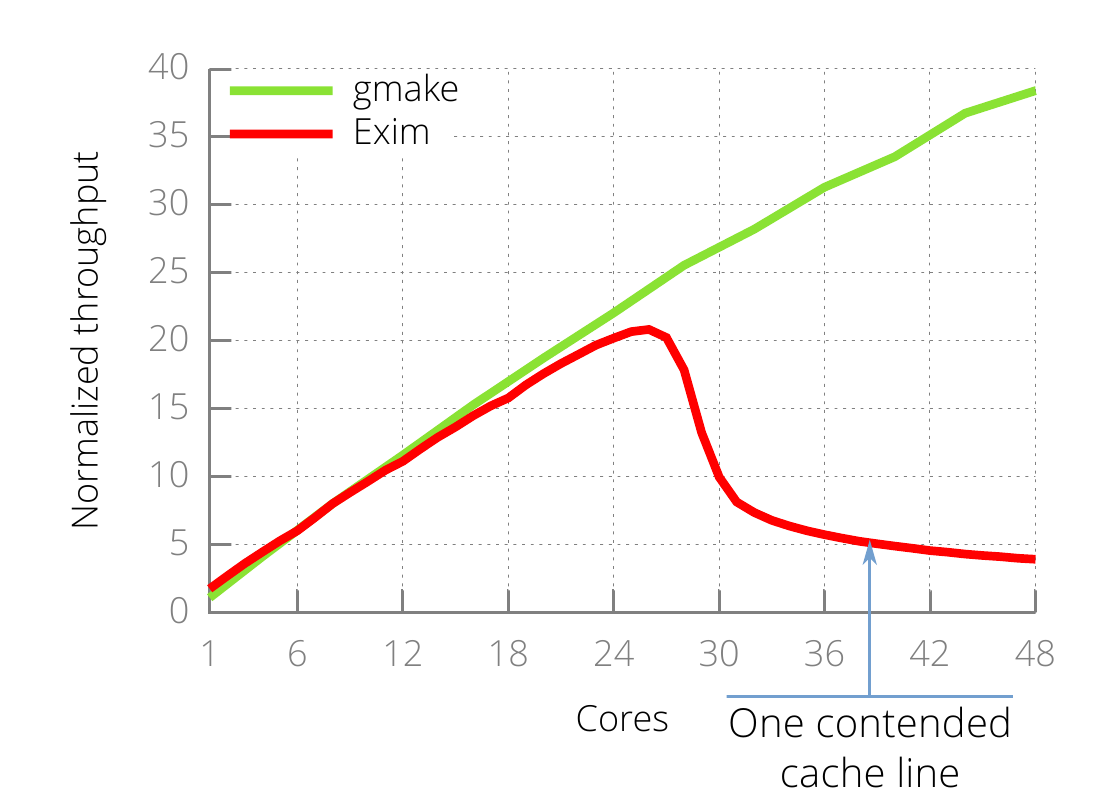
\includegraphics[width=0.8\textwidth]{799-s14-docs/cache_line_contention.png}
 \end{figure}

\footnotetext[1]{Figure borrowed from Clements' SOSP 2013 presentation}
\end{frame}

\begin{frame}
\frametitle{The scalability rule}
Assume a \uline{specification} $\mathscr{S}$ with a correct reference 
implementation M. Consider a \uline{history} $H = X || Y$ where $Y$ 
\uline{SIM-commutes} in $H$, 
and where M can generate $H$. Then there exists a correct implementation m of 
$\mathscr{S}$ whose steps in the $Y$ region of $H$ are conflict-free.
\end{frame}

\begin{frame}
\frametitle{Some teminology}

\begin{itemize}
\item A system execution is a sequence of \emph{action}s.
\begin{itemize}
\item An \emph{action}: either an \emph{invocation} or a \emph{response}.
\end{itemize}
\item A system execution is called a \emph{history}.
\begin{itemize}
\item \emph{Well-formed}: each thread's invocations and responses are in pairs.
\end{itemize}
\item The \emph{specification} distinguishes whether or not a history is 
  ``correct".
\item Reordering preserves the order of actions within each thread.
\begin{itemize}
\item $H|t = H'|t$ for every thread $t$.
\end{itemize}
\end{itemize}
\end{frame}


\begin{frame}
\frametitle{SIM-commutativity}

\begin{itemize}
\item $Y$ SI-commutes in $X||Y$ $:=$ \\
  $\forall Y' \in reorderings(Y), Z: X||Y||Z \in \mathscr{S} 
  \Longleftrightarrow X||Y'||Z \in \mathscr{S} $

\begin{itemize}
\item SI-commutativity considers reordering within a context prepared by 
previous operations (X) - state depedency.
\end{itemize}

\item $Y$ SIM-commutes in $X||Y$ $:=$ \\
  $\forall P \in prefixs(reorderings(Y)):$ P SI-commutes in $X||P$
\begin{itemize}
\item Monotonicity is needed to prove the theory.
\end{itemize}
\item SIM-commutativity is interface-based.
\end{itemize}

\end{frame}

\begin{frame}
\frametitle{SIM commutativity is state-dependent}

\begin{itemize}
\item It captures operations that commute in some states but not others.
\begin{itemize}
\item Few system calls unconditionally commute.
\end{itemize}

\item An example: two calls to \texttt{open("a", O\_CREATE | O\_EXCL)}
  \begin{itemize}
    \item Often don't commute.
    \item Commute if:
      \begin{itemize}
        \item different working directory;
        \item or if the file already exists. 
        \end{itemize}
\end{itemize}
\end{itemize}
\end{frame}

\begin{frame}
\frametitle{Come back to the scalable commutativity rule}
Assume a \uline{specification} $\mathscr{S}$ with a correct reference 
implementation M. Consider a \uline{history} $H = X || Y$ where $Y$ 
\uline{SIM-commutes} in $H$, 
and where M can generate $H$. Then there exists a correct implementation m of 
$\mathscr{S}$ whose steps in the \uline{$Y$ region} of $H$ are conflict-free.
\end{frame}


\begin{frame}
  \frametitle{Implementation terminology}
  \begin{itemize}
    \item An implementation $m$ is a function: $S \times I \longmapsto S \times R$
      \begin{itemize}
      \item S: system states
      \item I: invocations, including CONTINUE
      \item R: responses, including CONTINUE
      \end{itemize}
    \item An implemenation takes in an \uline{invocation} and outputs a 
      \uline{response}, and may modify the \uline{system state}.
  \end{itemize}
\end{frame}

\begin{frame}
\frametitle{Constructed non-scalable implementation}
\begin{multicols}{2}
\begin{figure}
   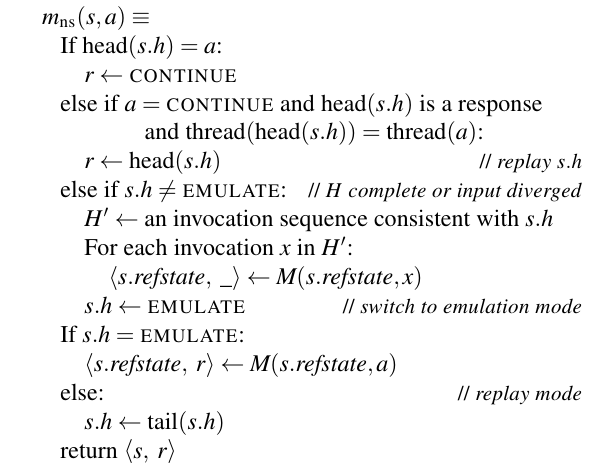
\includegraphics[width=0.45\textwidth]{799-s14-docs/nonscalable_imple.png}
 \end{figure}
\columnbreak
\begin{itemize}
\item Check the head of the history, if the call matches the invocation, replay.
\item Otherwise, use the reference implementation to emulate the system.
\end{itemize}
\end{multicols}

Not scalable because in replay mode, two threads conflict on accessing the history.

\end{frame}

\begin{frame}
\frametitle{Constructed scalable implementation}
\begin{multicols}{2}
\begin{figure}
   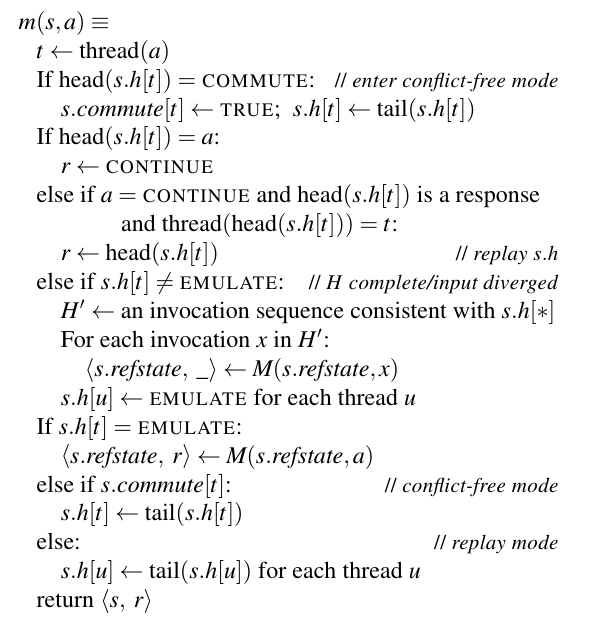
\includegraphics[width=0.45\textwidth]{799-s14-docs/scalable_imple.png}
 \end{figure}
\columnbreak
Each thread accesses only its thread-specific history - conflict-free.
\end{multicols}

How is SIM-commutativity used here?

\end{frame}

\begin{frame}
\frametitle{Discussion - is the rule actually useful?}
\begin{itemize}

\item The rule only says that a scalable implementation exists for a region in a
 particular history. But this history is not the only thing we use the system for.

\begin{itemize}
\item The authors: the arguments and system states for which a set of operations
 commutes often collapse into fairly well-defined classes. In practice, implemenations 
scale for whole classes of states and arguments.
\end{itemize}

\item Often a set of operations commutes in more than one class of situations, but no 
single implementation scales for all classes.

\begin{itemize}  
\item System designers need to understand the tradeoff.
\end{itemize}

\item Commutativity is not necessary for conflict-free accesses.
\item Some conflict-free accesses don't scale on real machines.

\begin{itemize}
\item Memory bus may get overwhelmed whether or not the accesses have conflicts.
\end{itemize}

\end{itemize}

\end{frame}

\begin{frame}
\frametitle{Designing commutative interfaces}
\begin{itemize}
\item Decompose compond operations
\begin{itemize}
\item \texttt{fork} vs. \texttt{posix\_spawn}
\item \texttt{stat}
\end{itemize}
\item Embrace specification non-determinism
\begin{itemize}
\item \texttt{open}, lowest available FD vs. any unused FD
\end{itemize}
\item Permit weak ordering
\begin{itemize}
\item \texttt{send, recv}
\end{itemize}
\item Release resources asynchronously
\end{itemize}
\end{frame}

\begin{frame}
\frametitle{Rest of the paper}
\begin{itemize}
\item \textsc{Commuter}
\item Apply \textsc{Commuter} to improve Linux.
\end{itemize}
\end{frame}

\begin{frame}
\frametitle{\textsc{Commuter}}
\begin{itemize}
\item Manually analyze the commutativity of an interface is tricky.
\item \textsc{Analyzer}
\begin{itemize}
\item Takes a symbolic mode of an interface and computes the conditions under which
the interface's operations commtue.
\item Considers every set of operations of a certain size (typically pairs). 
Uses symbolic execution to explore all possible paths.
\item At the end of a code path, checks if that path yeilds a result that's the 
same as other permutations of the operation.
\end{itemize}
\item \textsc{Testgen}
\item \textsc{Mtrace}
\end{itemize}
\end{frame}

\begin{frame}
\frametitle{\textsc{Analyzer} example input}
\begin{figure}
   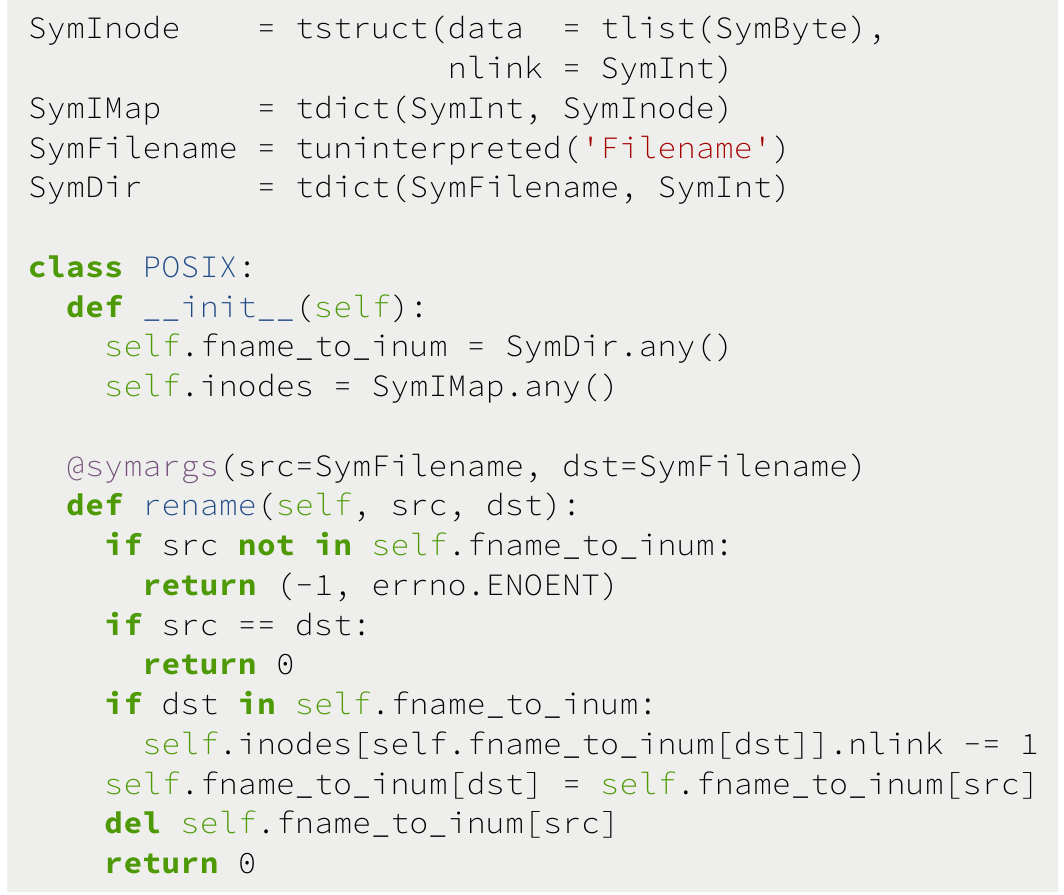
\includegraphics[width=0.8\textwidth]{799-s14-docs/commuter_rename.png}
 \end{figure}
\footnotetext[1]{Figure borrowed from Clement's SOSP 2013 presentation}
\end{frame}

\begin{frame}
\frametitle{\textsc{Commuter}}
\begin{itemize}
\item \textsc{Testgen}
\begin{itemize}
  \item Produces test cases to check if the implementation is actually 
    conflict-free when operations commute.
  \item Path coverage.
  \item Conflict coverage: the same path may result in different memory accesses.
  \item Start with the constraints of a path condition from \textsc{Analyzer}, 
    generates all possible concrete assignments for symbolic expressions 
    (negating equivalent assignments).
\end{itemize}

\item \textsc{Mtrace}
\begin{itemize}
\item Runs the test cases to check for conflicting memory accesses.
\item A modified QEMU.
\item Record memory accesses for each test case.
\end{itemize}

\end{itemize}
\end{frame}

\begin{frame}
\frametitle{Applying scalable commutativity rule to Linux}
\begin{itemize}
\item Linux 3.8 vs. sv6
\item 18 system calls
\item 13,664 test cases
\end{itemize}
\end{frame}

\begin{frame}
\frametitle{Results for Linux}
\begin{figure}
   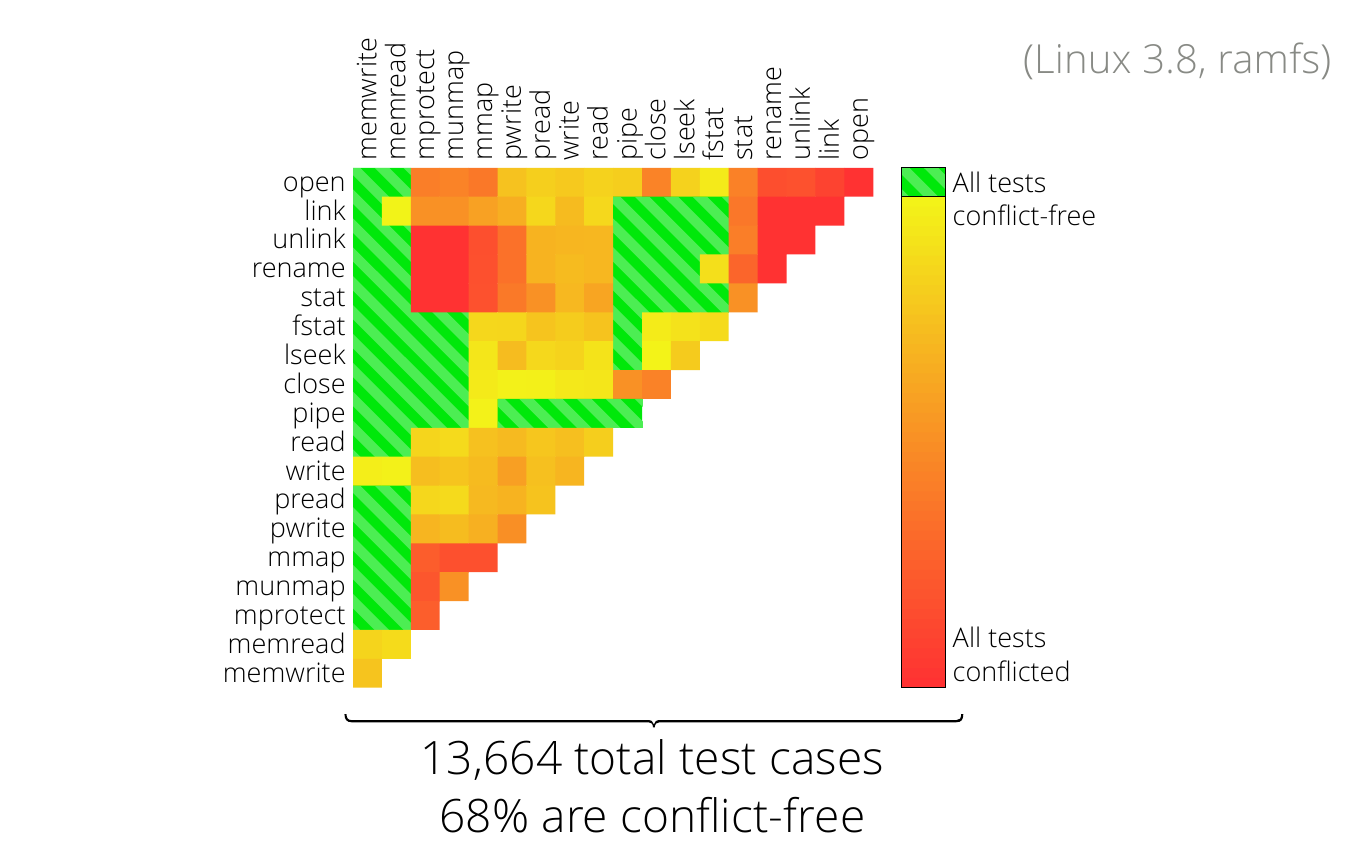
\includegraphics[width=\textwidth]{799-s14-docs/linux_result.png}
 \end{figure}
\end{frame}

\begin{frame}
\frametitle{Results for sv6}
\begin{figure}
   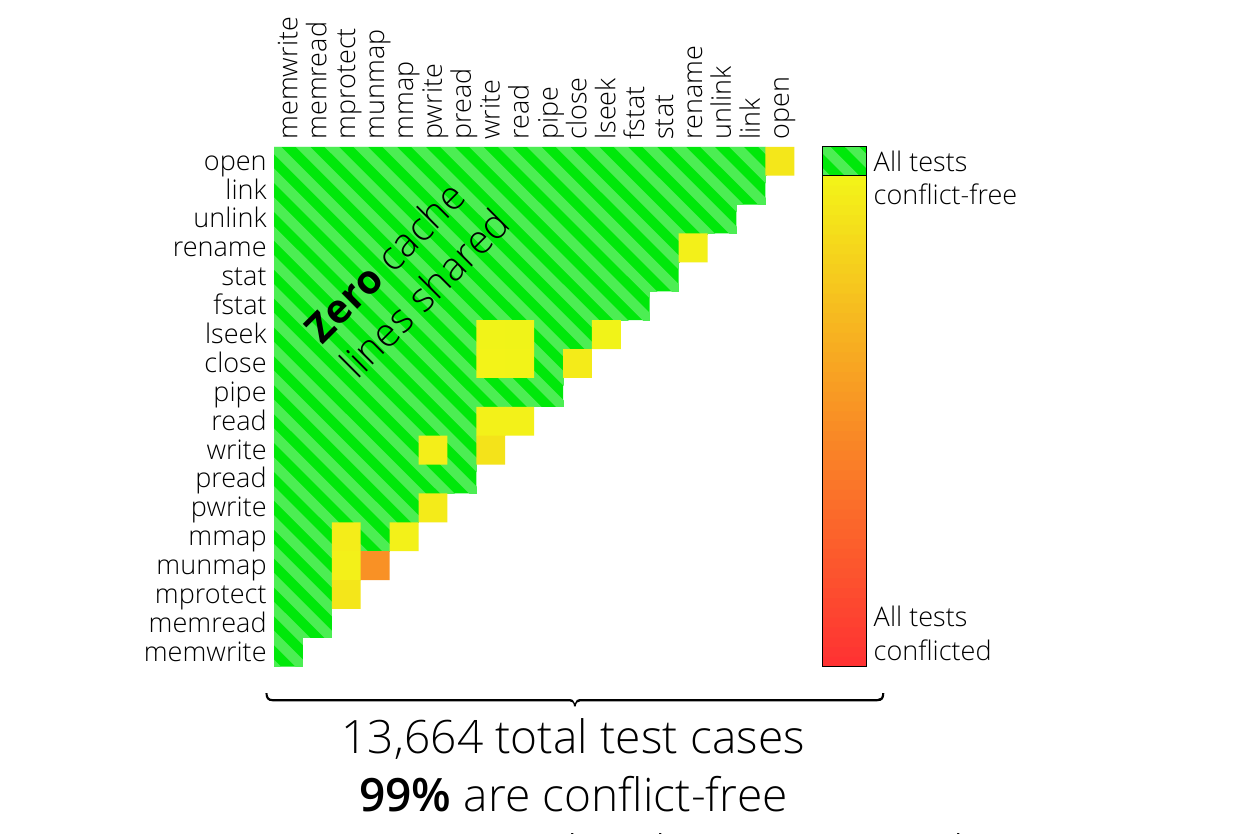
\includegraphics[width=\textwidth]{799-s14-docs/sv6_result.png}
 \end{figure}
\end{frame}

\begin{frame}
\frametitle{Making test cases scale}

\end{frame}

\end{document}

